\section{Ensaios de Envelhecimento}

Para induzir o fenômeno de BTI nos dispositivos foi utilizada uma câmara térmica para ensaios com componenentes eletrônicos. Inicialmente a temperatura de exposição foi de 100°C, temperatura que é inferior a faixa de ocorrência do BTI, mas que foi utilizada para verificar se os componentes não iriam ser danificados com a temperatura.

A Figura \ref{fig:CamTerm} mostra a câmera térmica utilizada para os ensaios. Ele foi fabricado pela SPX Thermal Product Solutions e alcança temperaturas de -75ºC a 200ºC.

\begin{figure}[H]
    \centering
    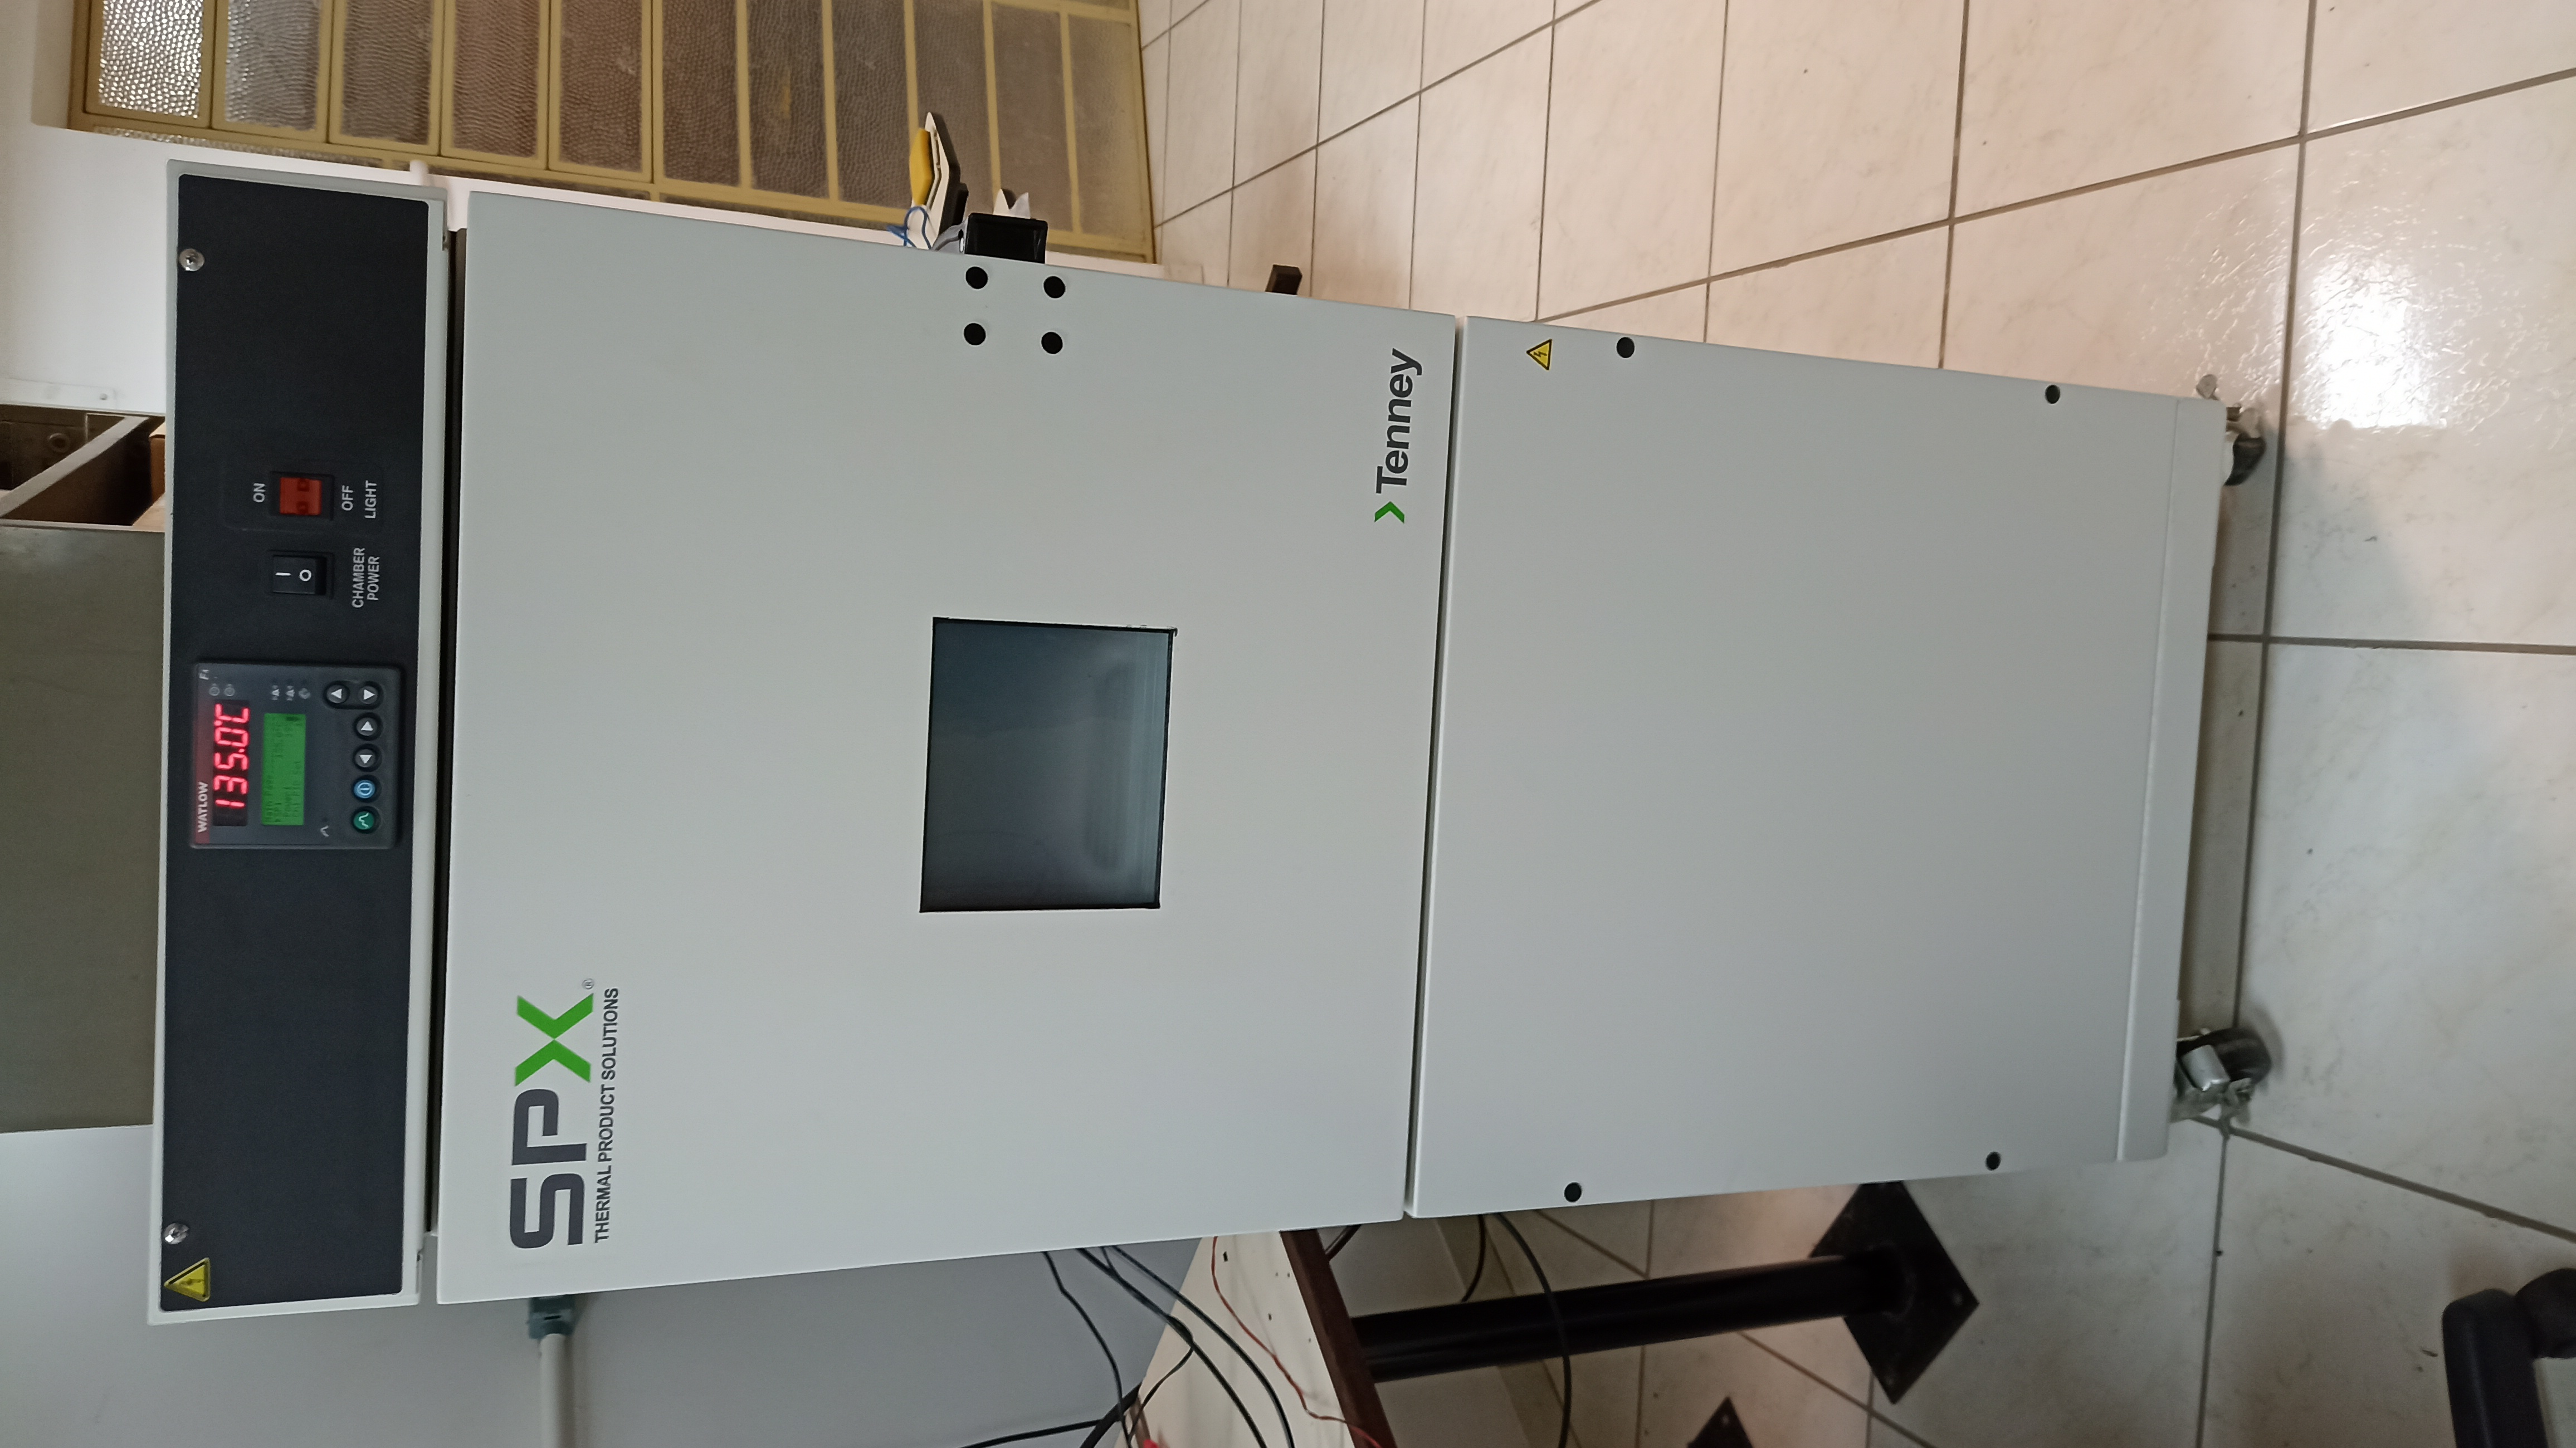
\includegraphics[angle=270, scale=0.08]{figures/Metodologia/Ensaios_CamaraTermica.jpg}
    \caption{Câmara térmica utilizada para os ensaios. Fonte: O Autor}
    \label{fig:CamTerm}
\end{figure}

Constatando que não houve problema à 100ºC, a temperatura foi aumentada para 125°C. Como também não houve danos, a temperatura foi, então, elevada para 135°C.

Nessa temperatura foi observado que o conector de alimentação da placa DE2 apresentava sinais de derretimento, por isso, a temperatura dos ensaios foi definida em 135°C. Temperatura que está dentro da faixa de 125 e 175ºC que a bibliografia indica como sendo a faixa em que o BTI ocorre mais facilmente.

O tempo total de estresse térmico foi de 150h, tempo definido levando-se em conta o que foi estudado na seção \ref{sec:GerandoNbti}. A contagem do tempo era iniciada quando a câmara térmica era ligada e paralisada quando desligada.

O tempo que os dispositivos foram expostas ao calor não foi contínua, devido a impossibilidade de ficar durante a noite no laboratório e, por motivos de segurança, de deixar a câmara térmica ligada sem supervisão. Portanto os dispositivos, de forma geral, foram expostos à câmara térmica durante o dia e retirados dela durante a noite, ficando ligados o tempo todo, de forma que não houvesse relaxamento.

Outras duas placas, dos mesmo modelos das ensaiadas, foram deixadas fora da câmara térmica pelo mesmo tempo, sempre ligadas e com os mesmos osciladores em anel sintetizados. Comparar as medidas entre as placas que foram aquecidas com as que não foram é importante para verificar que se a degradação na frequência é proveniente do estresse térmico ou se é apenas resultado do funcionamento prolongado.

A câmara térmica permite realizar medidas nos dispositivos ensaiados enquanto eles estão dentro dela. Portanto foi possível medir a frequência dos osciladores em anel durante o processo de estresse térmico. As Figuras \ref{fig:CamTerm} e \ref{fig:Osciloscopio} mostram o setup experimental construído, com os FPGAs ensaiados dentro da câmera térmica com os cabos de medição saindo da câmera e ligadas ao osciloscópio.

\begin{figure}[H]
    \centering
    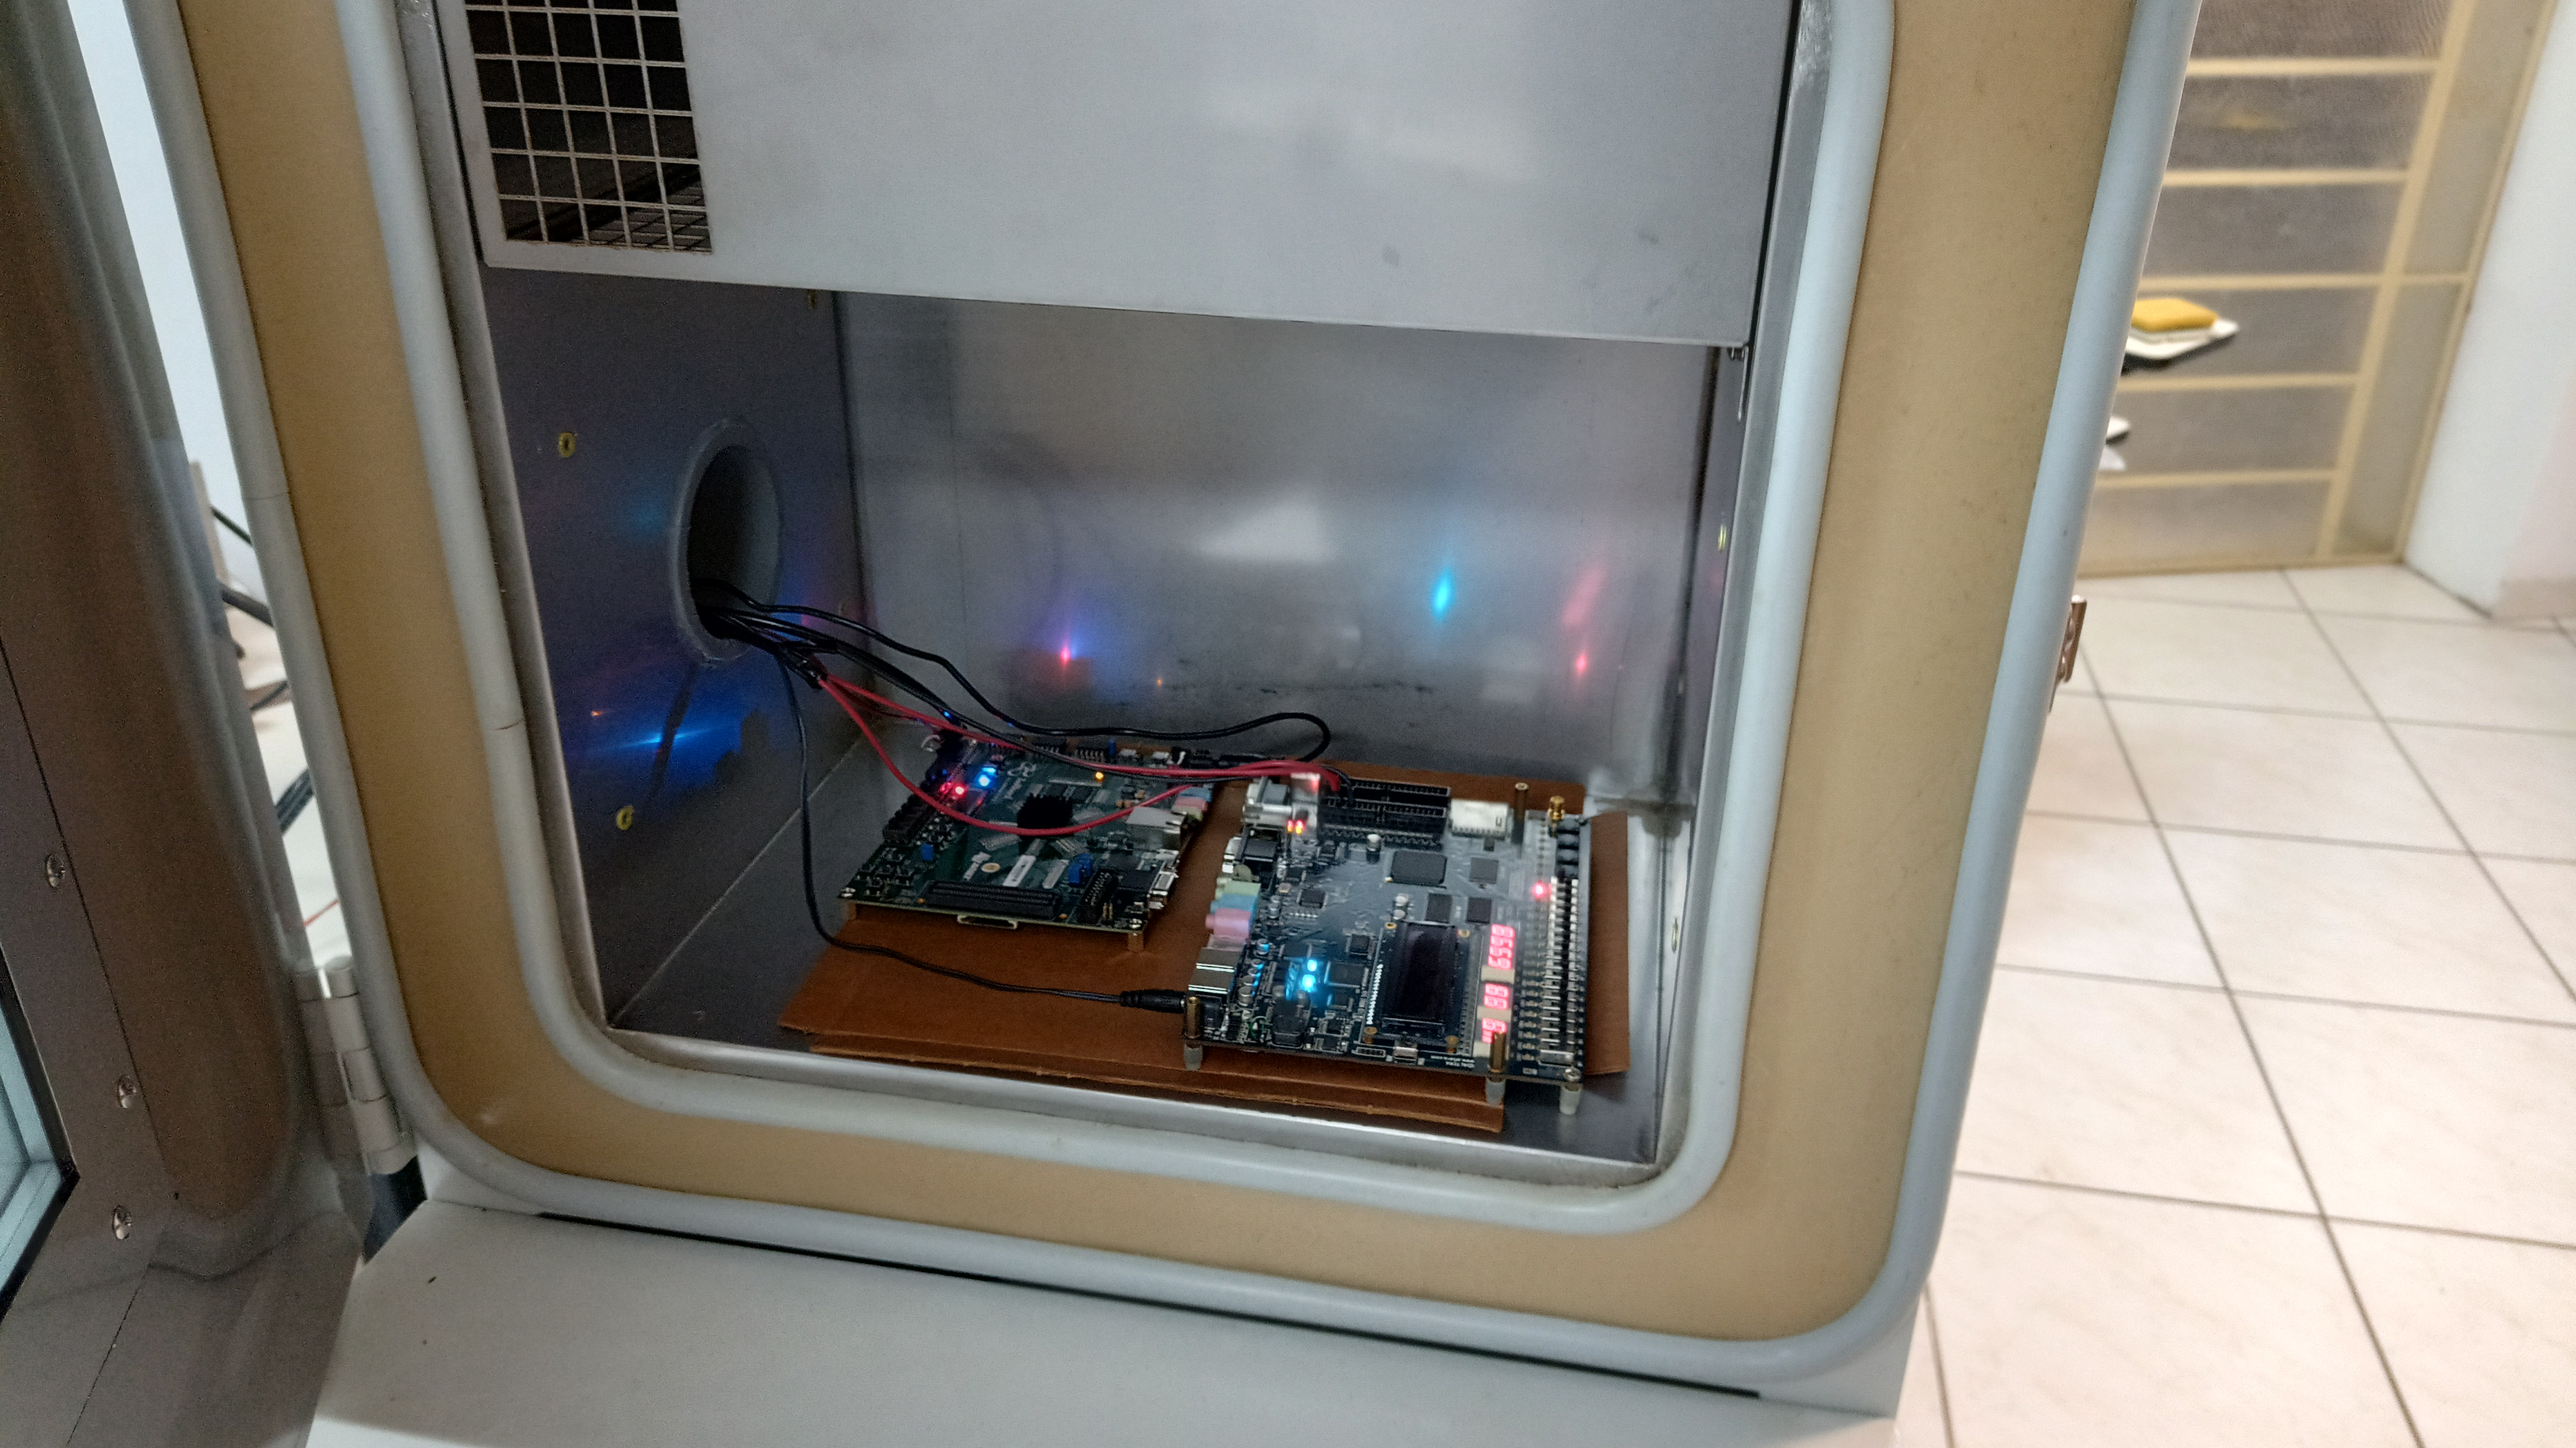
\includegraphics[width=\linewidth]{figures/Metodologia/Ensaios_FpgasNoForno.jpg}
    \caption{FPGAs dentro da Câmara térmica. Fonte: O Autor}
    \label{fig:CamTerm}
\end{figure}

\begin{figure}[H]
    \centering
    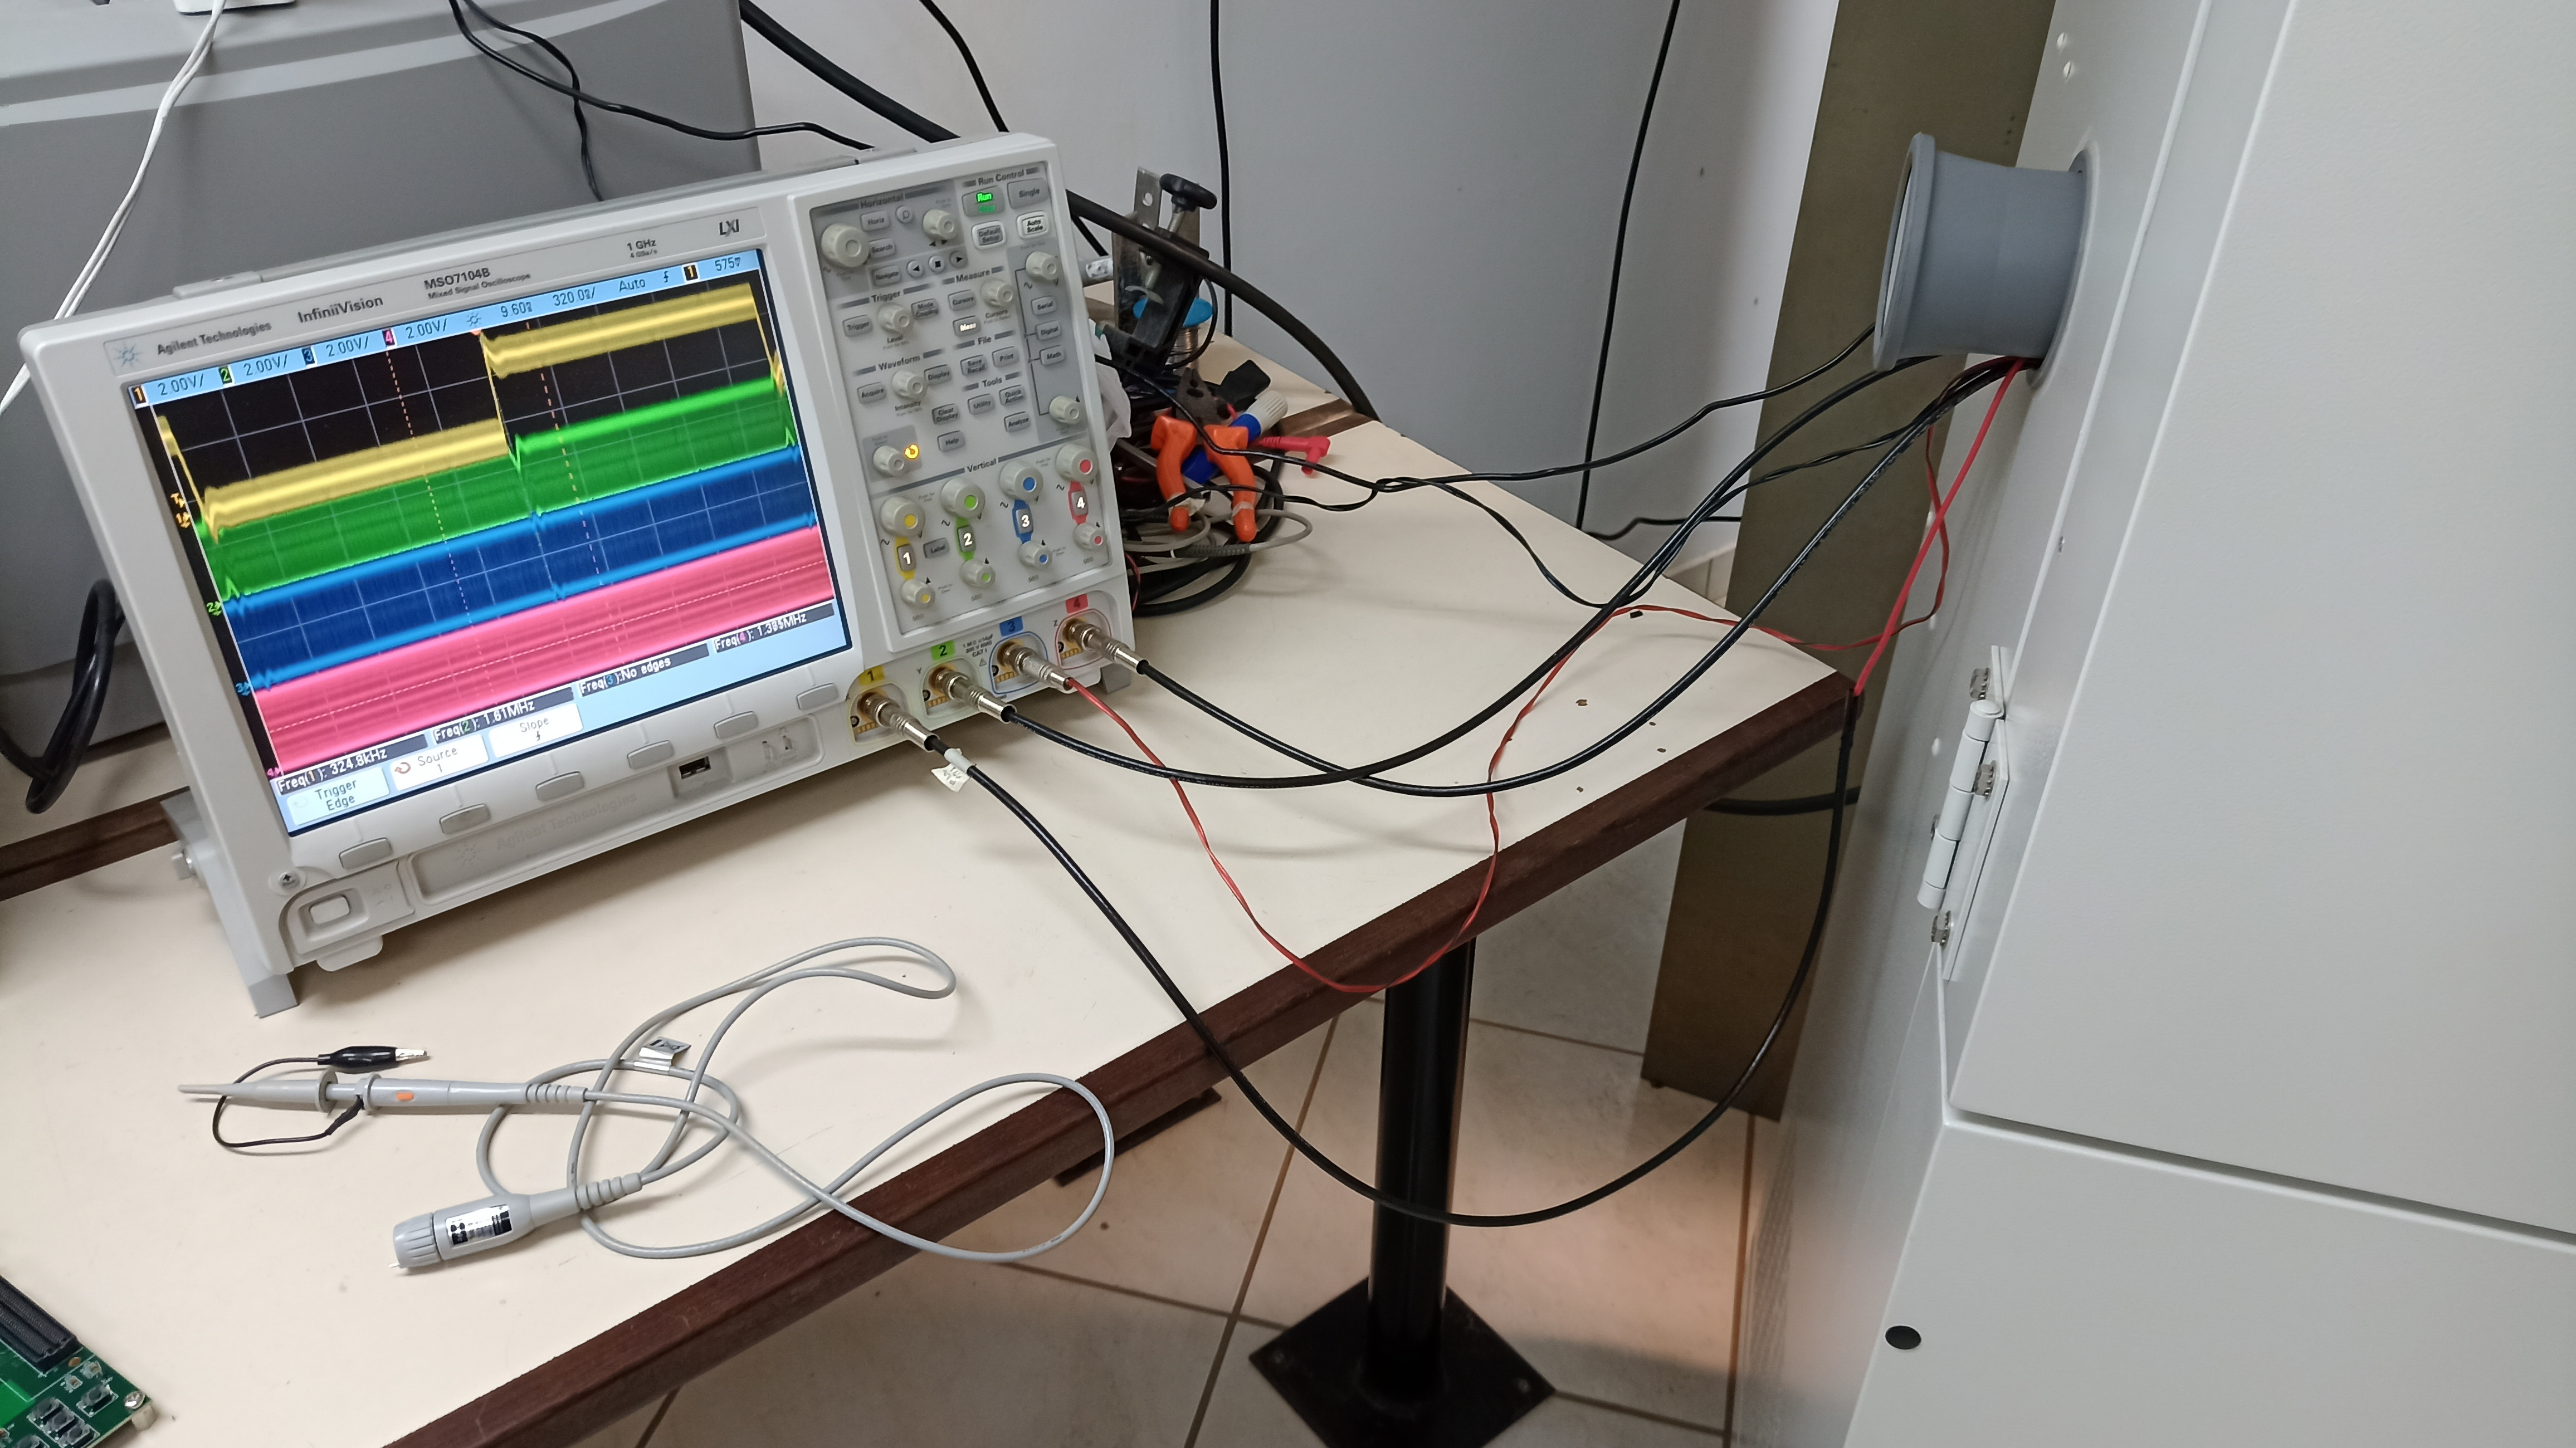
\includegraphics[width=\linewidth]{figures/Metodologia/Ensaios_Osciloscopio.jpg}
    \caption{Osciloscópio utilizado para as medidas. Fonte: O Autor}
    \label{fig:Osciloscopio}
\end{figure}

Enquanto a câmara aquecia da temperatura ambiente para a temperatura alvo, as medições foram mais frequentes, mantendo-se, no máximo um período de cinco minutos entre as medidas. Quando a temperatura alvo é atingida as medidas ficam mais esparsas, considerando que há menos variação na frequência medida.

É importante separar os efeitos instantâneos da temperatura na frequência dos osciladores do efeito a longo prazo do BTI. Por isso é necessário comparar as medidas feitas em uma mesma temperatura. O momento que a temperatura é a mais estável é quando a câmara já chegou aos 135°C.

Com as medidas ao longo do aquecimento da câmara é possível construir curvas de frequência por temperatura e compará-las para diferentes ciclos. Como em cada ciclo os dispositivos estão há um determinado tempo sofrendo estresse, será possível analisar o deslocamento dessa curva, se houver, com o passar do tempo.

Comparando essas medidas em relação ao tempo total estressado será possível constatar se houve ou não uma degradação na frequência de funcionamento dos dispositivos, e se houve uma diferença significativa na degradação entre as duas placas.

Após os ensaios de envelhecimento foi realizado um ensaio para medir a recuperação dos circuitos, para verificar quanto da degradação sofrida é reversível. Para isso as quatro placas foram desligadas e deixadas em temperatura ambiente. Medidas ao longo do tempo foram realizadas até o tempo de relaxamento totalizar o tempo total que as placas foram estressadas.
